\chapter{Introduction}
\label{ch:intro}
\chaptermark{Introduction}

%\setcounter{equation}{0}
% ==========================================================================================================
\newpage
% ==========================================================================================================
\section{Mind wandering as a heterogeneous phenomenon}
\sectionmark{Heterogeneity}
In the past decade, mind wandering has gained wider interest in science. Researchers aim at understanding how the mind shifts between external environment and internal thoughts unrelated to the here-and-now. The study of mind wandering roughly fall into two categories, the characteristic of mind wandering (i.e. how human mind wanders.) and the processes that generate it (i.e. why human mind wanders.). Both aspects are essential of the study of mind wandering. However, the two approaches have led to a conflict in the study of mind wandering in various aspects. 

\subsection{Heterogeneity in definitions}
In past years, mind wandering has been studied in a variety of related psychological domains, such as cognition, emotion, and neuroscience. Various lines of research have addressed the basic phenomenal characteristics of mind wandering---
\begin{quote}
    \textit{a shift in the contents of thought away from an ongoing task and/or from events in the external environment to self-generated thoughts and feelings.}\\    
    \cite{SmallwoodSchooler2006,SmallwoodSchooler2015}.
\end{quote}
We can all find moments when the train of thought shift away from the tasks at hand, and sometimes getting annoyed by the mind wandering episode. The intuition has lead to researches describing mind wandering as an `attention lapse' \cite{McVayJOEP2009, McVay2012}, implying the occurrence of mind wandering is an unintended failure. When the study explicitly instruct the participant to perform a task, the time not focusing on the task are considered as `mind wandering'. Such research design dismissed the possibility of voluntary engagement of the mind wandering state. 

Recent investigations have found that mind wandering can occur with or without intention \cite<see review from>{SeliTiCS2016}. 
The participant can, however, intentionally mind wander if they lack a motivation to engage in the experiment. When a simple yes/no question is asked about the mind wandering state, the response cannot access the nature of the occurrence. When participants are asked about the nature of mind wandering period in laboratory scenario, a proportion of the mind wandering period is intentional. The reason behind intentional mind wandering  could be the lack of motivation to complete the task
\cite{SeliJoEP2015}
, or the task is not mentally demanding to have all the attention resource allocated to the task \cite{SeliPsychScience2016}. 
The occurrence of intended and unintended mind wandering can also be down to individual differences. 
Intentional and unintentional mind wandering have been found to be deferentially associated with attention-deficit/hyperactivity disorder \cite<ADHD;>{SeliADHD2015} and obsessive-compulsive disorder \cite<OCD;>{SeliOCD2017}. More fine-grained investigation on the commonality of mind wandering will help resolve the conflict in the definition.

\subsection{Heterogeneity in functional outcomes}

Although mind wandering is a common occurrence in our day-today life, the functional consequence remains poorly understood \cite{SmallwoodFrontiers2013, Mooneyham2013}. Mind wandering has been considered the reason of poor executive control during working memory task \cite{McVayJOEP2009}. Individuals who mind-wandered more during fluid intelligent testing perform less well \cite{MrazekJoEP2012}. Mind wandering leads to bad reading comprehension due to failure in the construction of the mental models of ongoing events \cite{Smallwood2008}. Comprehension ability is related to working memory capacity and mediated by the ability to suppress mind wandering \cite{McVayReading2012, Unsworth2013}. Mind wandering has been linked to unhappiness \cite{Killingsworth2010} and a indicator of depression \cite{Smallwood2007}. The evidence above supported the highly disruptive nature of mind wandering and its potential costs to cognitive performance.

In addition to exploring the costs of mind wandering, researchers have discovered its potential benefits. Mind wandering may facilitate creative solution to an old problem \cite{Baird2012, Smeekens2016} and recovery from negative emotional states \cite{RubyPlos2013, PoerioFrontiers2016}. Mind wandering relays on mental time travel---the metal capacity of remembering the past and imagining the future \cite{Stawarczyk2015}.  Mind wandering can refine personal goals \cite{Medea2016} and is associated with the neural mechanism supporting mental time travel \cite{DArgembeau2006,DArgembeau2015}. 

The wide-range of associated functional outcomes suggests mind wandering is not a homogeneous state. To reconcile this contradictory evidence, researchers have suggested that mind wandering may be heterogeneous, encompassing multiple states with differential contents and underlying cognitive architectures \cite{SmallwoodFrontiers2013}. Different functional associations arise from different `types' of experience, which explains the range of functional outcomes observed in the literature.


\subsection{Heterogeneity in experiential profiles}
Self-report is commonly used to understand the content of mind wandering thoughts and on-going experience. The content of mind wandering has a wide variety of topics and modality. Studies using principle component analysis (PCA) have revealed more detailed experiential profiles. Temporal information is one common theme \cite{RubyFP2013,RubyPlos2013}. The content of mind wandering is mainly future-focused \cite{Baird2011}, therefore mind wandering often involves planning for the future goals of the individual. On the contrary, when the mind wanders in an unhappy mood, the content is drawn to events from its past \cite{Smallwood2011}. The form of spontaneous thoughts is likely to be imagery or verbal \cite{Gorgolewski2014,Smallwood2016}. Investigations in experiential profiles is the first step into explore the commonality of various type of mind wandering. However, the link between different experiences and the cognitive aspect is not yet well described.  


% ==========================================================================================================

\section{Theoretical accounts of mind wandering}
\sectionmark{Theoretical accounts}

Although mind wandering is both a cause of error in external tasks and unhappiness, it is also a correlate of creativity and personal problem solving. In addition, it is a correlate of both greater and lesser executive control. The discovery on mind wandering can be formalised into two theoretical accounts. The executive failure account aim to understand the conditions that trigger or associate with mind wandering. Researches on the mechanism behind the occurrence of mind wanderings is the representational account. In other words, the executive failure account examines why mind wandering happens, while the representational account interests in how human mind wanders. The differences in research interest illustrates how two accounts develop conflicting views of mind wandering. 

\subsection{Executive failure account}
The executive failure account emerges from researches linking mind wandering and problems maintaining a task relevant goal in mind. Mind wandering occurs during attention-demanding tasks when control processes are insufficient to deal with the interference created by off-task thoughts \cite{Kane2012,McVay2010}. Mind wandering results from a failure of executive control over internally generated thoughts, rather than as consuming executive resources. The researches focus on the negative effect of mind wandering on the development of negative mood and task performance. Mind wandering thoughts are mostly unhappy in ecologically valid scenario \cite{Killingsworth2010}. Depressive thinking correlates with the frequency of mind wandering \cite{Smallwood2007}. Mind wandering has been considered the reason of poor executive control during working memory task\cite{McVayJOEP2009}. Executive error and slow reaction time correlates with individual differences in working memory capacity and mind wandering \cite{McVay2012}. The capacity to avoid mind wandering during demanding tasks is a potentially important source of success on measures of fluid intelligence \cite{MrazekJoEP2012}. 

% neural basis
In the executive failure view, mind wandering reflects momentary lapse in attention. Task-based functional magnetic resonance imaging (fMRI) study on attention lapse has contributed the functional neural processes to support the executive failure account. \citeA{Weissman2006} have uncover the neural mechanism behind the attention lapse during a global/local selective-attention task. The definition of attention lapse is a relatively slow response time to the task at hand, which is consistent with the mind wandering indicator used in working memory capacity research \cite{McVay2012}. Brief attention lapse is related t early activity in frontal control region including anterior cingulate cortex (ACC), right middle frontal gyrus (MFG), and right inferior frontal gyrus (IFG). Attention laspse also suggested the failure of maintaining perceptual representation. Reduced activity is found in primary visual area. Activation of default mode network \cite<DMN; >{Raichle2001} has been observed during a brief attention lapse. DMN is a set of brain regions composed of medial prefrontal cortex(MPFC), and posterior cingulate coretex (PCC) as the core and subsystems on medial and lateral regions of the temporal lobe. DMN is commonly referred as a task-negative network\cite{Fox2005}, associating with task-unrelated thought and mind wandering \cite{MasonScience2007,Christoff2009}. The lapses leads to demands on the frontal-parietal control relate regions for redirecting attention. Ventral frontal-parietal regions, including right temporal-parietal junction (TPJ) and right IFG, for recovery from lapses. 

\subsection{Representational account}

The representational account explores the generation of on-going thought during mind wandering, with the emphasis on the contribution of memory and its neural basis. Content of thoughts relies on episodic/semantic memory to represent the on-going thought \cite{Binder2009,Gusnard2001}. Semantic memory refers to an internal knowledge system about the world acquired through experience. Human relies on efficient manipulation of semantics memory to solve problems, achieve goals, and reason abstract logic. Episodic memory describe the collection of past personal experiences that occurred at a specific time and space. The representational account helps explain psychological studies on creativity \cite{Baird2012,Smeekens2016} and social-temporal problem solving \cite{RubyPlos2013,PoerioFrontiers2016,Medea2016}. The poor executive function results from resource competition in the representational view of mind wandering \cite{SmallwoodSchooler2006}. Mind wandering can be a resource prioritisation of internal memory representation over the external environment, explaining the productive functional outcomes on future planning \cite{Baird2011} and creativity \cite{Baird2012}. 

Internal representation of semantics and episodic memory is supported by studies in functional neuroimaging. The brain regions involved in semantic processing includes angular gyrus (AG), lateral and ventral temporal cortex, left dorsal MPFC, left IFG, left ventral MPFC, PCC \cite<see meta-analysis from >{Binder2009}. Dorsal and ventral MPFC show high activity at rest and are associated with personal relevant information\cite{Gusnard2001}. PCC has been proposed as the integrational hub of information from medial and lateral temporal lobe \cite{Smallwood2016}.  Integration of the hippocampus with the DMN facilitates mental time travel \cite{Karapanagiotidis2017}. The ability for these regions to become functionally decoupled from perception dominant systems allows them to operate in an offline manner \cite{Smallwood2013,Schooler2011}. Process of decoupling may also be important in neural systems closely allied to those involved in memory. These transmodal system potentially facilitating their role in stimulus independent aspects of cognition \cite{Buckner2013,Margulies2016,Mesulam1998}.

% ==========================================================================================================
\section{Neural hierarchies}
\sectionmark{Neural hierarchies}

The two accounts of mind wandering are stemmed from distinctively different psychological research approach to understand mind wandering. However, the related neural systems involves the same set of system---the attention system and the DMN---interacting in a seemly contradicting manner. In the executive failure account, the attention-related system deactivates with poor task performance, accompanied by the activation in the DMN; while in the the representational account, the attention system and the DMN works to gather to maintain the internal representation of memory. The speculation is that the global neural hierarchy has different configuration to serve different purposes. In the current section, I discuss the progress of functional neuroimaging study towards a hierarchical view of neural systems corresponding to the two contradicting account of mind wandering.

\subsection{Historical perspective}
The idea of functional specialisation in brain has a long standing history dating back from the proposal of phrenology in the \nth{19} century. 
\cite{Kanwisher2010}

% network
\cite{Sporns2014}

\cite{Mittner2016}

\cite{SmallwoodFrontiers2013}

% gradient
\cite{Margulies2016}

\subsection{Abstract rules governing}
\cite{Duncan2010}

\cite{Fox2005}

\cite{Weissman2006}

\subsection{Sensory integration}
\cite{Mesulam1998}

\cite{Villena-Gonzalez2018}

\cite{Murphy2018}


\subsection{Compensation}
\cite{VatanseverPNAS2017}

\cite{Crittenden2015}

\cite{Crittenden2016}

% ==========================================================================================================
\section{Towards a better account of mind wandering}
\sectionmark{The current thesis}

The conflicts in the mind wandering literature arise for the heterogeneous, unconstrained nature of mind wandering. To date, the mind wandering researches consist of investigations on three important aspects: experience, neural profile, and cognition (Fig.\ref{fig:intro:fig1}). A detailed description for the spontaneous thought is needed to confirm the experience during mind wandering. Neural organisation serves as the intrinsic biological basis of cognition. Finally, established cognitive measures link the functional outcome to the experiential profiles. Studies targeting relationships of a singular aspect and mind wandering. To paint the full picture of mind wandering, a multivaritate method will help incorporate the three aspects. 

The current thesis adapts a multivariate approach as the first step towards a new view on mind wandering. Multidimensional experience sampling \cite<MDES; >{Medea2016, RubyPlos2013, Smallwood2016} is the main technique of experience profile assessment. Resting state functional connectivity is used to describe the trait-like neural feature of each individual. The tasks selected measure cognitive functions documented in the past mind wandering literature, including executive control, fluid intelligence, episodic memory, semantic memory, and information generation. Finally, canonical correlation analysis \cite<CCA; >{Hotelling1936} is the conjoined-decomposition method of choice to explore the multivariate patterns of mind wandering. Here I present the overview of the mind wandering measure and the benefit of CCA used in the thesis.  

\subsection{Content of experience}

\begin{wrapfigure}{o}{0.5\textwidth} 
	\centering
	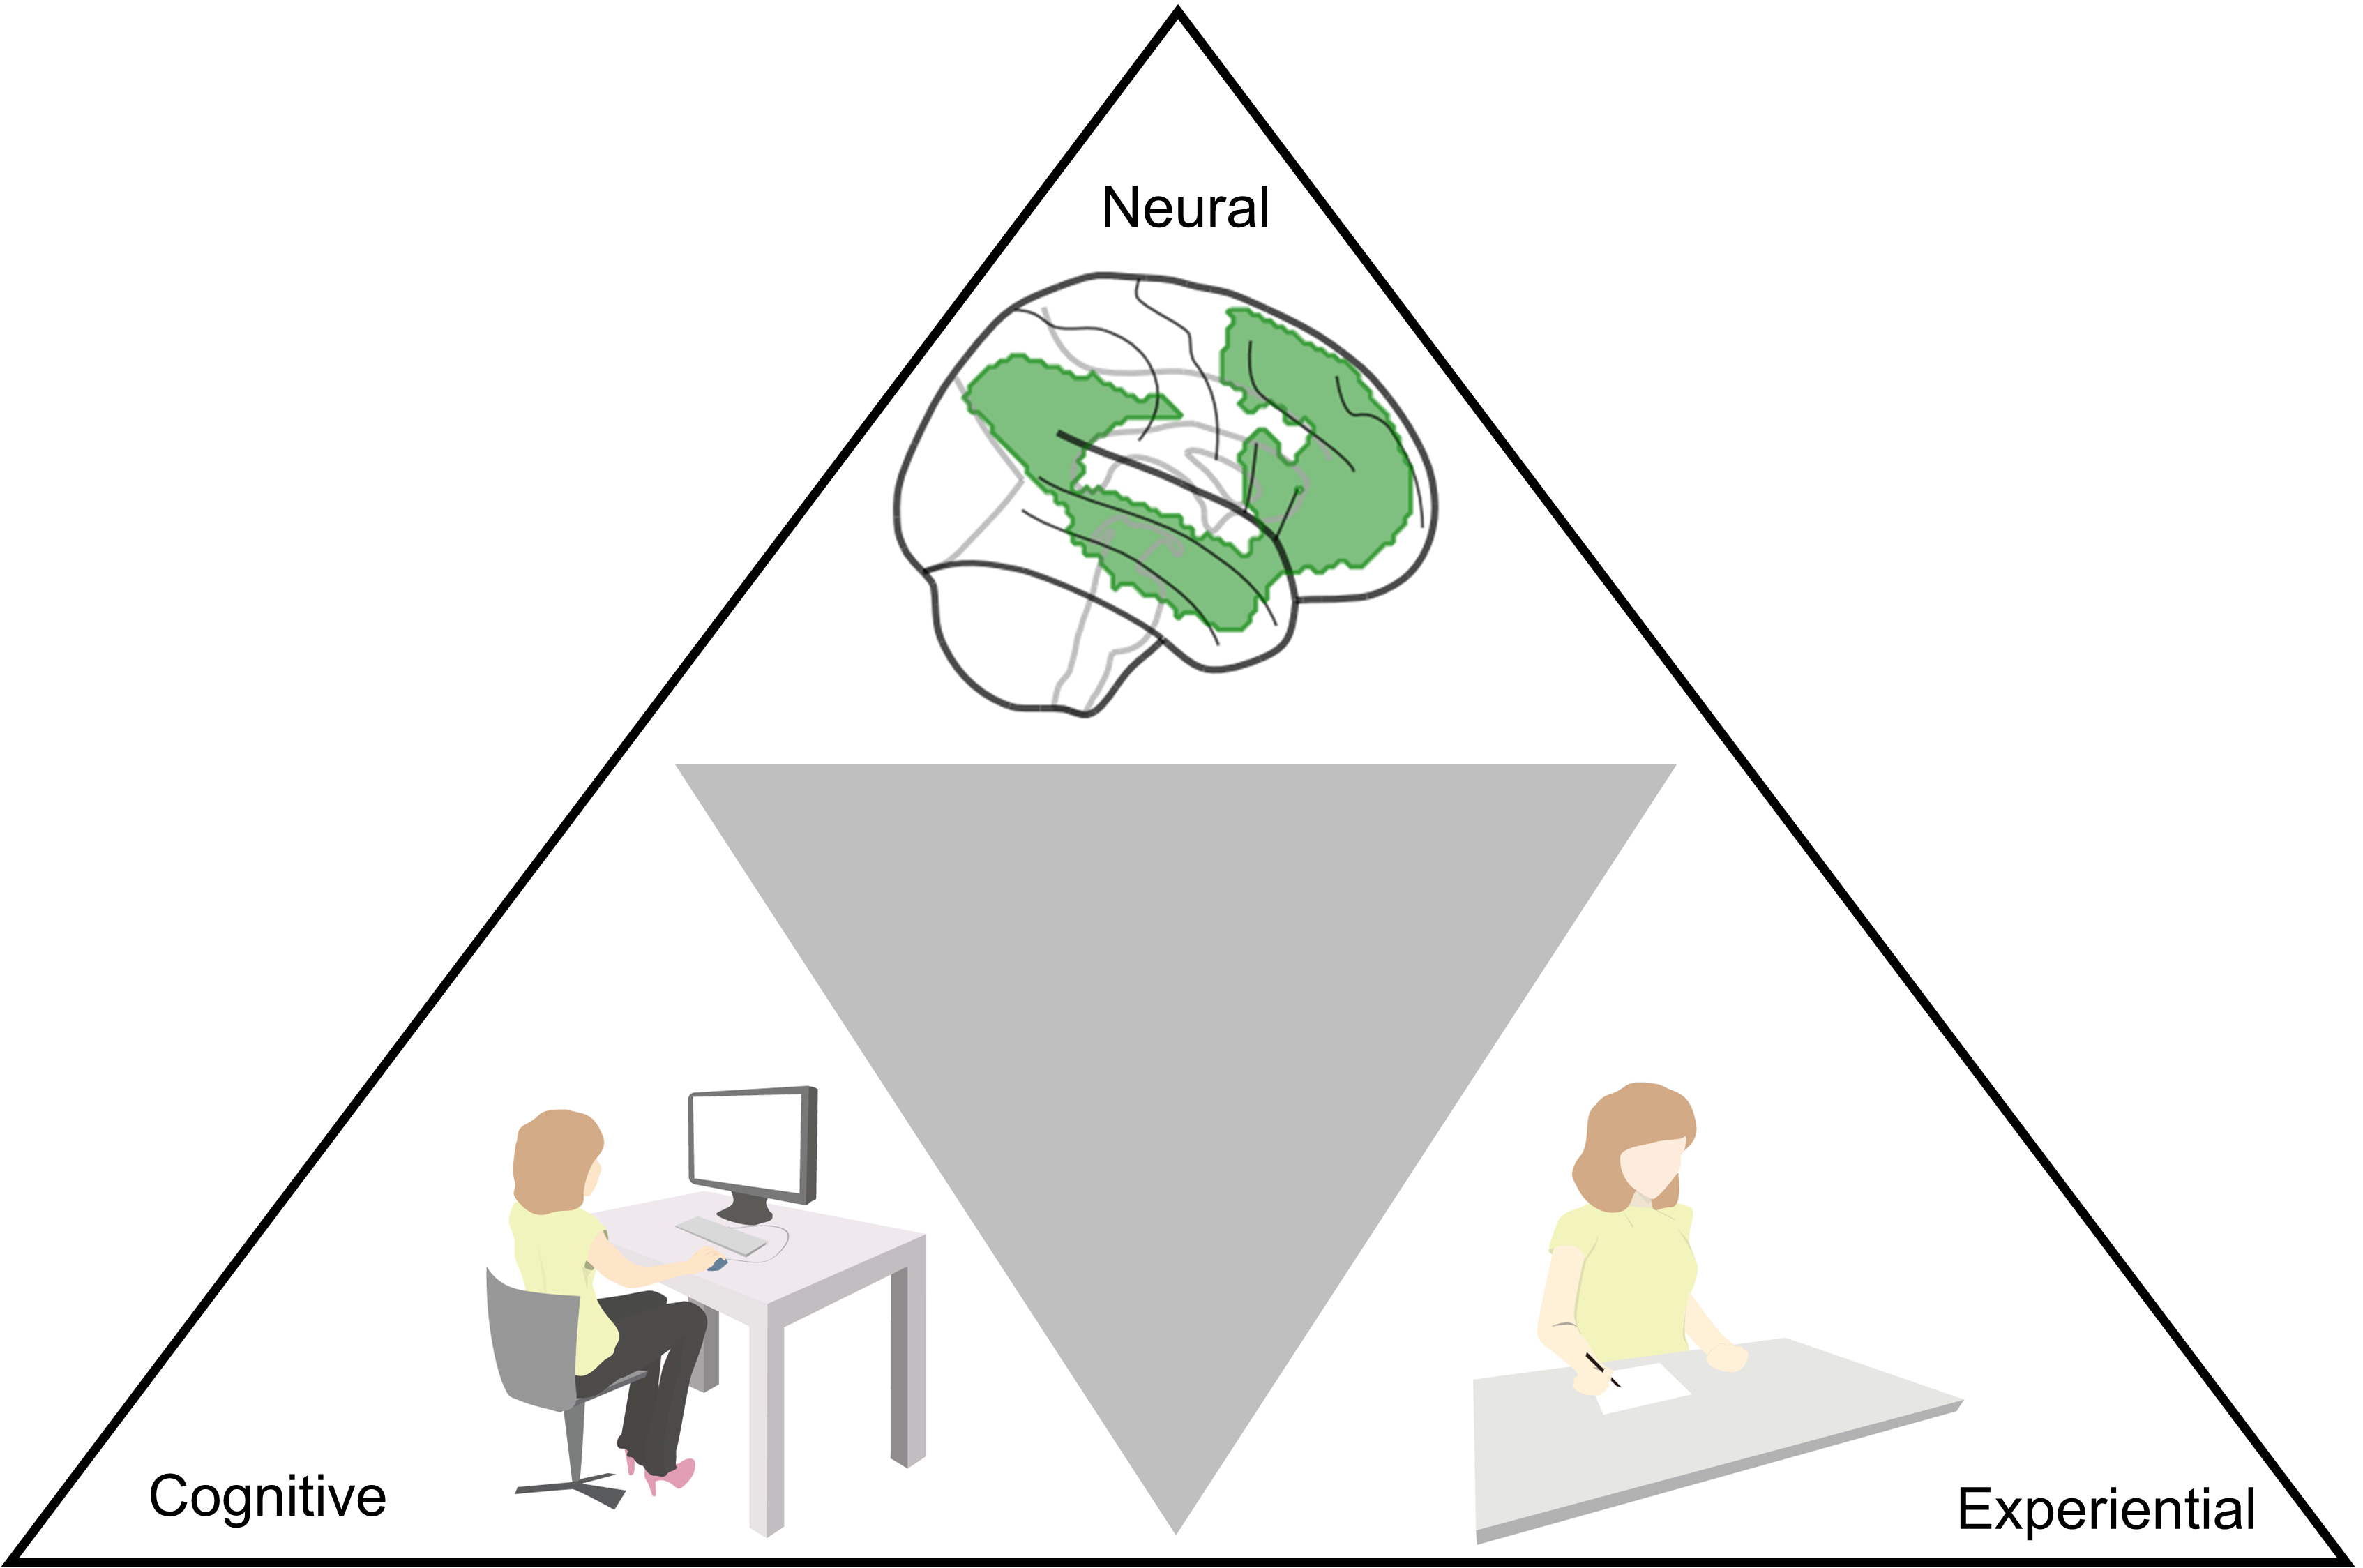
\includegraphics[width=0.48\textwidth]{chapters/img/thesisfig1.png}
	\caption{Schematic of the thesis}
	\vspace{-20pt}
	\label{fig:intro:fig1}
\end{wrapfigure}

To access the complex, heterogeneous content of spontaneous thoughts, the current thesis employs MDES \cite{Medea2016, RubyPlos2013, Smallwood2016}. For the purpose of capturing momentary evolution of thoughts during experiments, experience sampling \cite{Kahneman2004} is the commonly used technique. MDES expanded the thought probe from a on/off task question to a collection of dimensions related to a wide range of form and content of thoughts. The idea of MDES is based on various questionnaires to understand the content of mind wandering thoughts retrospectively, such as the Dundee Stress State Questionnaire \cite{Matthews1999}, Amsterdam Resting-State Questionnaire \cite{Diaz2013}, the resting state questionnaire \cite{Delamillieure2010}, and New York Cognition Questionnaire \cite{Gorgolewski2014}. The questionnaires above involves more than 20 items, providing a comprehensive coverage of thought content. Direct implementation of the retrospective questionnaires listed above is not practical for experience sampling. Experience sampling is conducted along an external task, such as reading \cite{Franklin2011}, go/no-go task \cite{Christoff2009}, and n-back task\cite{Kane2007}. The list of questions need to be short and concise to minimum interruption of the external task.

The current version of MDES is based on 10-question set used in \cite{Medea2016} and \citeA{Smallwood2016}. In the previous work, the questions are separated into content and form aspect of experience. Principle component analysis (PCA) was used to extract latent linear structure in the spontaneous thought report. Each participant has a set of identified principle components concluding the average momentary state of all the sampled time period. The current version includes both form and content questions in one set with three extra questions. The average score of each thought dimension indicate the average momentary state of spontaneous thought.

\subsection{Method of acquiring experience}

In the current thesis, both online and retrospective method are used to acquire content of mind wandering in laboratory scenario. In the second empirical study, New York Cognition Questionnaire \cite{Gorgolewski2014} is used to acquire the trait-like multidimensional mind wandering thought content during a 9-minute resting state fMRI session. The retrospective method measures the summary of the mind-wandering experience during a specified time period. The benefit of retrospective measure is that no interruption during the given task or the on-going thoughts will happen. The trait-level features of mind wandering are accessed in the retrospective report. 

In the online measure, MDES serves as the thought probes to record participant's experiences during a give task. A hybrid of go/no-go task and n-back task was used to manipulate working memory capacity to induce mind wandering \cite{Konishi2015, Medea2016}. The earlier version has used number as the test items \cite{SmallwoodNI2013,SmallwoodPlos2011}. The majority of the experiment consist of nontarget presented in neutral colour and a small proportion of targets. The participant are instructed to judge whether the target number is odd or even. In the \textit{choice reaction time} (i.e. 0-back) condition, the judgement is made when the number changes colour; in the \textit{working memory} (i.e. 1-back) condition, participants judge the number on the previous screen when presented with a question mark. The improved version is proposed by Konishi and colleagues \citeyear{Konishi2015}, replacing number with two 2-dimensional geometric shapes separated by a vertical line. Each pair consists of a two shapes among a circle, a triangle, and a square, each in two different left/right configurations. In the 0-back condition, the target is flanked by one of two shapes, and participants indicate which shape matches the target shape. In the 1-back condition, the target is flanked by two question marks, and participants match the target shape to the prior trial. Thought probe appears during the task in a semi random fashion. The online measure captures spontaneous thought in, possibly, both mind-wandering and task-focused moments. In the first and third empirical studies, the averaged momentary report from MDES is used to capture the trait-like feature of spontaneous cognition.

\subsection{Conjoined decomposition of brain and cognition}

Despite invented in the 30s, CCA has not aroused researchers’ interests due to the lack of practicality. With the advance on computing resource and enriched data size, CCA has gained popularity in neuroimaging research. Three characteristic of CCA make it the choice of method---joint information compression, symmetry, and multiplicity (details described in the Method chapter). CCA can be understood as a natural extension of PCA to two variable sets, but mutually linked by a joint correlation criterion. Such extension enables the exploration of neuro-experiential component pairs of mind wandering. CCA does not distinguish between the two variable sets during the information compression process. The identified dual-component dimensions correlates two aspect the data together without indication of causality between neural function and cognition. CCA is capable of estimating more than one corresponding component pair from the two variable sets. More than one pair of meaningful decomposition can be found, giving it the potential to examine the heterogeneity of mind wandering content and their functional outcome. 

While CCA provided useful features to explore the heterogeneity of mind wandering, its sparsity variation overcomes two technical issues of CCA application. Performing feature selection with sparsity improve the interpretability of the data and model fit. The data with more number of features than samples is accompanied with consequences of the so-called curse of dimensionality---the more dimensions are added to a data set, the less explanatory value a sample would have \cite{Domingos2012}. The number of functional connectivity measure can easily exceed the number of samples. In sum, SCCA allows decomposition on functional connectivity measures without sacrifice of data richness or interpretation difficulty of prior data compression. The pros and cons of CCA and its variation is disccussed in the next chapter.

The current thesis adopt the sparse variation of CCA \cite<SCCA; >{WittenSCCA2009} to resolve arguments related to heterogeneity in mind wandering. Most studies in mind wandering have only focused on its relationship with one cognitive outcome at a time. As a consequence, mind wandering is treated as a singular construct. Studies on contents of spontaneous thoughts have shown the diversity of information using self-report methods. Based on the heterogeneity of content of spontaneous thoughts, mind wandering can be a collection various type of spontaneous thoughts. Adopting multivariate method has the potential to identify family resemblance among the heterogeneity of mind wandering, and to begin the research on the ontological view of mind wandering. 

% ==========================================================================================================
\section{Summary and thesis outline}
\sectionmark{Summary}
The mind wandering is a common human experience. Human cognition has the capacity to generate thoughts loosely related to the external world. However, researchers have not understood the mechanism behind the consequences of mind wandering. The heterogeneity of functional outcomes has been a controversial and much disputed subject within the field of mind wandering research. Extensive research has shown that both cost and benefit to cognitive functions are associated with mind wandering. Negative consequences include reduced attention, poor task performance, unhappiness, and depression.  The related positive outcomes include creative problem solving, planning personal goals, and recovery from negative emotion. 

Most studies in mind wandering have only focused on one cognitive outcome at a time. Mind wandering is treated as a singular construct. Studies on contents of spontaneous thoughts have shown the diversity of information using self-report methods.  The temporal content of spontaneous thoughts can be future- or past-focused. The topic can be on personal issues or task related. Based on the heterogeneity of content of spontaneous thoughts, mind wandering can be a collection various type of spontaneous thoughts. The lack of specificity in thought content could result in conflicts in the functional outcome of mind wandering literature.

In the past decade, the neural basis of mind wandering has become the centre of the topic. Default mode network (DMN) is the commonly emerged large-scale network. Extensive literature have documented the task-negative trait of DMN. The executive failure account of mind wandering is in line with the task-negative view of DMN. However, the memory representation aspect of the mind wandering mystery is left unresolved. Recent literature on the neural hierarchy has shade a different light on the function of DMN. The high-level cognitive functions are associated with DMN, whereas perception and motor related regions are related to low-level tasks. This new view provides a clue to investigate the representational account of mind wandering. 

The conflict in mind wandering literature is related to the one-to-one matching between mind wandering and the brain or behaviour. To paint the full picture of mind wandering, a multivaritate method will help incorporate the three aspects mentioned above: cognition, experience, and neural basis. The current thesis adopt canonical correlation analysis (CCA) to resolve arguments related to heterogeneity in mind wandering. Despite invented in the 30s, CCA has not aroused researchers’ interests due to the lack of practicality. With the advance on computing resource and enriched data size, CCA has gained popularity in neural imaging research. The motivation of the current thesis is to resolve the conflict in mind wandering literature incorporating functional organisation of large-scale neural networks. The aim is to present evidence supporting the heterogeneity of mind wandering and to begin research on the ontological view of mind wandering. A outline of the remaining chapter is listed below: 

\section*{Canonical correlation analysis}

Canonical correlation analysis is introduced as the main method of the thesis. This review focuses the potential applications in neuroimaging research. The features, applications of this multivariate method are outlined, followed by discussion on the method's the interpretations and limitations. 

\textit{This chapter is under preparation for publication. } 

\section*{Study 1}
Heterogeneity of mind wandering leads to conflicts in its functional outcome in behavioural study. Default mode network is commonly associated with the emergence of mind wandering. Sparse CCA conjointly decomposed functional connectivity patterns of DMN and thought reports, revealing unique neuro-experiential components. The study then revealed that the neuro-experiential components each associate with unique cognitive task measures. The various connectivity configuration within DMN is associated with different types of mind wandering and their specific functional outcomes.

\textit{This chapter is published in Psychological Science.}

\section*{Study 2}
Unconstrained cognitive processes have two faces. The representational account argues that the primary sensory brain region decoupling from the DMN to facilitate memory representation; whereas the executive failure account shows lapses in attention is related to the demand to attention system and activation of DMN. Mind wandering is an unconstrained cognitive state, therefore we used sparse CCA to extract related whole brain functional connectivity patterns, profiling the neuro-experiential components of unconstrained cognitive processes. Examining the association between demanding cognitive tasks and neuro-experiential components, the study revealed evidence supporting both the representational and executive failure accounts.

\textit{This chapter is published in NeuroImage.}

\section*{Study 3}
Various cognitive function is involved in the generation of internal experiences. The study of the functional outcome are often conducted in a manner of one-to-one mapping. The heterogeneous cognitive outcomes are discussed as conflicts rather than the complex details driving the diversity of mind wandering. In the current chapter, we explore the intrinsic whole-brain neural basis of the cognitive functions supporting the unconstrained generation of spontaneous thoughts.  With sparse CCA we describe the conjoined decomposition of cognitive function and resting state functional connectivity. The study explore the unconstrained neruocognitive mechanism underlying the various dimensions of spontaneous thoughts.

\section*{Discussions}
The overarching themes of the thesis are discussed and linked to specific results throughout the thesis. Future research directions are inspired by the findings and limitations of the current thesis.

% ==========================================================================================================
